% simulations
We use simulations to provide additional evidence for theoretical claims and to gain insight into audit behavior. As in \cite{simulations}, we use margins from the 2020 US Presidential election---state-wide pairwise margins of 5\% or more between the two leading candidates. Narrower margins are computationally expensive, especially for the simulations of tied elections, which, by design, have a low probability of stopping and hence quickly increase in sample size. We use the simulator in the R2B2 software library\cite{r2b2_anon}. For each margin, for each hypothesis, we perform $10^4$ trials. All trials use a $10\%$ risk limit, a maximum of $5$ rounds, and a conditional stopping probability of $0.90$ in each round. That is, each subsequent round size is selected to be large enough, assuming the announced tally is correct and given the tally of previous rounds, to give a $0.90$ probability of stopping in the current round.

\begin{figure}
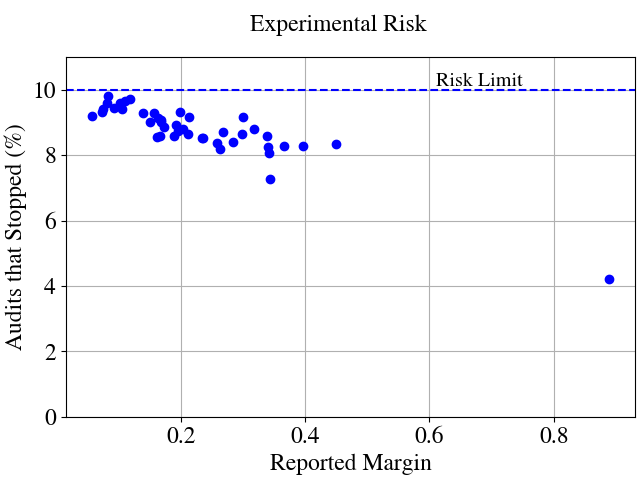
\includegraphics[width=.5\textwidth]{prov_risk.png}
\caption{The fraction of simulated \Providence audits on tied elections that stopped in any rounds (we performed five rounds at a $10\%$ risk limit). This value is an estimate of the maximum risk of the \Providence audit.}
\label{fig:prov-risk}
\end{figure}

In the simulations of \Providence audits of a tied election, the fraction of audits that stop, as shown in Figure~\ref{fig:prov-risk}, is an estimate of maximum risk. For all margins, this estimated maximum risk is less than the risk limit, supporting the claim that \Providence is risk-limiting.

\begin{figure}
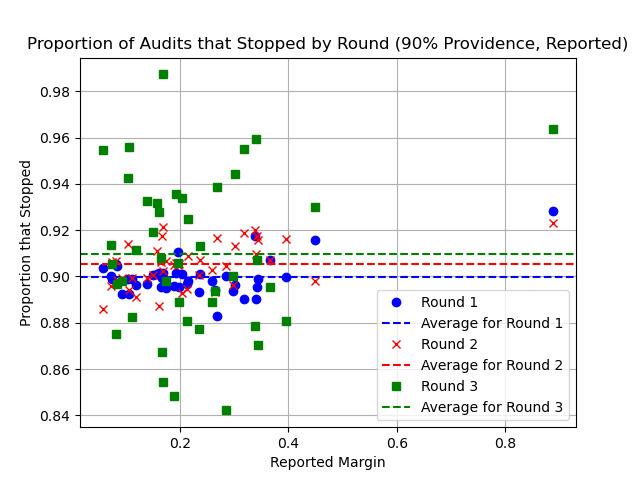
\includegraphics[width=.5\textwidth]{prov_sprob.png}
\caption{The fraction of simulated \Providence audits of the election as announced that stopped for each round. This value is an estimate of the stopping probability conditioned on the sample of the previous round. The average fraction for rounds 1, 2, and 3 is $89.96\%$, $90.52\%$, and $90.98\%$ respectively. We show only the first three rounds since so few audits make it to rounds 4 and 5.}
\label{fig:prov-sprob}
\end{figure}

Simulations of audits of the election as announced provide insight into stopping probability and number of ballots drawn when the election is as announced. We wish the stopping probability to be as predicted, and the number of ballots drawn to be small. Figure~\ref{fig:prov-sprob} shows that the stopping probabilities over the first rounds are near and slightly above $90\%$ as expected since our software chose round sizes to give at least a $90\%$ conditional stopping probability.

Figure~\ref{fig:prov-asn} plots the probability of stopping as a function of the number of ballots sampled. Points above (higher probability of stopping) and to the left (fewer ballots) represent more efficient audits. As shown, \Providence has comparable efficiency to \Minerva, while both are significantly more efficient than either implementation of \BRAVO. In a contest with a narrow margin (in the 2020 US Presidential election, eight states had margins less than $3\%$) the difference in number of ballots sampled could correspond to many days of work. 
% Section~\ref{sec:workload} discusses workload in more depth.

\begin{figure}
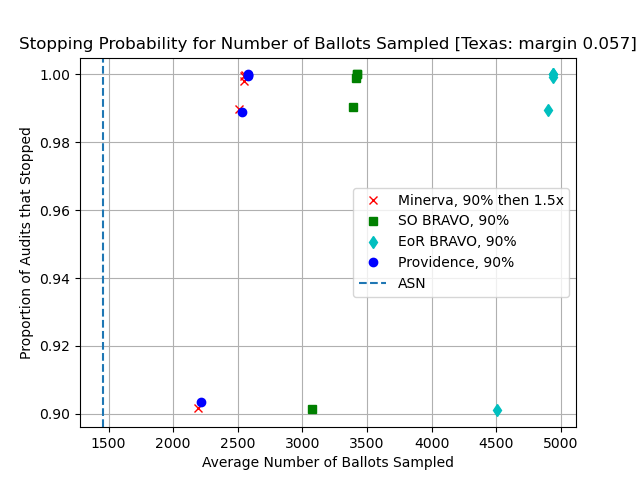
\includegraphics[width=.5\textwidth]{prov_asn.png}
\caption{For the entire audit, consisting of all five rounds, the estimated stopping probability for average number of ballots drawn for \Providence, \Minerva, EoR \BRAVO, and SO \BRAVO. The average sample number (ASN) for \B \BRAVO is included for context.}
\label{fig:prov-asn}
\end{figure}








